\documentclass{article}
\usepackage[utf8]{inputenc}
\usepackage{datetime}
\usepackage{enumerate}
\usepackage{textcomp}
\usepackage{amsmath}
\usepackage{tikz}
\usetikzlibrary{arrows}

\title{\bf \Large ASSIGNMENT 1}
\author{Xinhao Luo}
\date{\today}

\def\math#1{$#1$}

\setlength{\textheight}{8.5in}
\setlength{\textwidth}{6.5in}
\setlength{\oddsidemargin}{0in}
\setlength{\evensidemargin}{0in}
\voffset0.0in

\begin{document}
\maketitle
\medskip

\section{Problem 1.40 }
\begin{enumerate}
    \item Since we are about to acquire two gumballs(for two kids) with same color, the worst case is that we have brought three times and each time we have gumballs with different colors: 1 red, 1 blue, and 1 green. However, the next time we will only have a gumballs within these three colors, and it satisfied the 2 gumballs with same color condition. The number of money will be spent under such condition will be \math{1 \times 4 = 4} cents.
    \item If there are four children, which we need 4 gumballs with same color. In worst case, we will have to buy all red and blue gumballs before we get the 4 green gumballs, so we have to be willing to buy all 10 gumballs in the machine if we want to achieve this goal, and that is \math{1 \times 9 = 9} cents.
\end{enumerate}

\section{Problem 2.5(a)}

\math{(A \cap C)\cup(A \cap B)}

\section{Problem 2.21(c)}

\math{V = \{x|x = {(-1)}^{(n+1)} \times n; \ where \ n \in \mathbb{Z}, n \geq 0\}}

\section{Problem 2.22(c)}

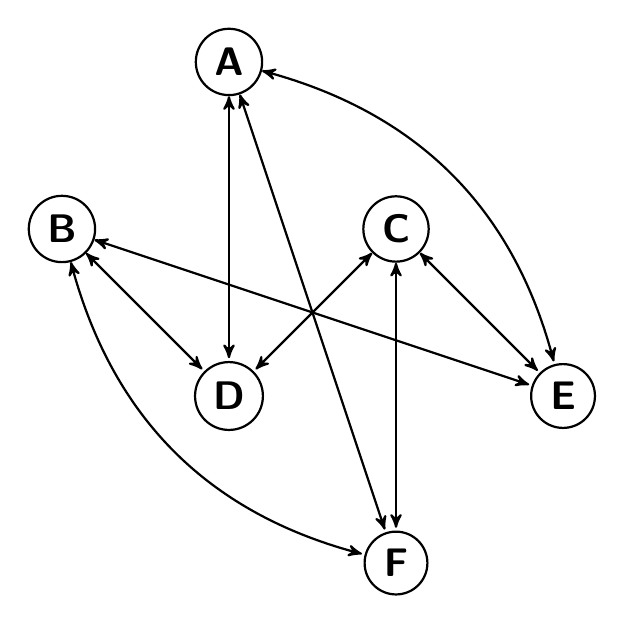
\begin{tikzpicture}[<->,>=stealth',shorten >=1pt,auto,node distance=3cm,
                    thick,main node/.style={circle,draw,font=\sffamily\Large\bfseries}]

  \node[main node] (1) {A};
  \node[main node] (2) [below left of=1] {B};
  \node[main node] (3) [below right of=1] {C};
  \node[main node] (4) [below right of=2] {D};
  \node[main node] (5) [below right of=3] {E};
  \node[main node] (6) [below right of=4] {F};

  \path[every node/.style={font=\sffamily\small}]
   (1) edge node [left] {} (4)
   (2) edge node [right] {} (4)
   (3) edge node [right] {} (4)
   (1) edge [bend left] node {} (5)
   (2) edge [left] node {} (5)
   (3) edge [right] node {} (5)
   (1) edge [right] node {} (6)
   (2) edge [bend right] node {} (6)
   (3) edge [left] node {} (6);
\end{tikzpicture}

\section{Problem 3.9}

\begin{enumerate}
  \item Equivalent statement is: If I eat peas, I will get ice-cream.
  \item No.
  \item No, parents are not required to give ice-cream.
\end{enumerate}

The statement made by parents is totally different from the one children imagine. To be specific, parents does not define the result after eating peas. If \textit{I} do eat peas, we could have ice-cream, but \textit{I} will never get if \textit{I} don't.

\section{Problem 3.13}

\textbf{Answer: At least 3; Card with P, 3, 4}
\begin{center}
    \begin{center}
    \textbf{Truth table}
    \end{center}
    \begin{tabular}{|c|c|c|}
    \hline
    p  & q  & \math{p \to q} \\
    \hline
    T  & T  & T \\
    T  & F  & F \\
    F  & T  & T \\
    F  & F  & T \\
    \hline
    \end{tabular}
\end{center} 

For the discussion below, 
\begin{enumerate}[i.]
    \item Set \math{p} to be \textit{Card with P}
    \item \math{q} will be \textit{Card's side with 5}.
\end{enumerate}

Since we need to prove this rule is true, it is saying that \math{p \to q} is true.

Based on the \textbf{Truth table, row 2}, The only way to falsify this statement is: \math{p} is true while \math{p} is false.

In this case, we need to 
\begin{enumerate}
    \item flip \textit{Card with P} (\math{p}), prove \math{q} is false.
    \item flip \textit{Card with 3 and 4} (\math{q}), prove \math{p} is true.
\end{enumerate}

\section{Problem 3.23}

\subfloat Truth table 1 {
    \begin{tabular}{|c|c|c|c|}
    \hline
    p &  q &  r & \math{((p \land q) \to r)} \\
    \hline
    F &  F &  F &  T \\
    F &  F &  T &  T \\
    F &  T &  F &  T \\
    F &  T &  T &  T \\
    T &  F &  F &  T \\
    T &  F &  T &  T \\
    T &  T &  F &  F \\
    T &  T &  T &  T \\
    \hline
    \end{tabular}
}
\subfloat Truth table 2 {
    \begin{tabular}{|c|c|c|c|}
    \hline
    p &  q &  r & \math{((p \lor q) \to r)} \\
    \hline
    F &  F &  F &  T \\
    F &  F &  T &  T \\
    F &  T &  F &  F \\
    F &  T &  T &  T \\
    T &  F &  F &  F \\
    T &  F &  T &  T \\
    T &  T &  F &  F \\
    T &  T &  T &  T \\
    \hline
    \end{tabular}
}
\\\\\\
For the discussion below, 
\begin{enumerate}[i.]
    \item \math{p} is set to \textit{ace the quiz}
    \item \math{q} is set to \textit{ace the final}
    \item \math{r} is set to \textit{get an A}
    \item Assume all \textit{If...Else...} statements are true
\end{enumerate}
Problems: 

\begin{enumerate}[(a)]
    \item I don't know. \\
\math{q} is true. Based on the \textbf{Truth Table 1}, this situation matches row 3, 4, 8, while \math{r} can either be true or false.
    \item Yes. \\
\math{q} is true. Based on the \textbf{Truth Table 2}, this situation matches row 4, 8, and \math{r} in both conditions are true.
    \item I don't know. \\
\math{r} is true. Based on the \textbf{Truth Table 1}, this situation matches row 2, 4, 6, 8, and \math{q} here can either be true or false.
    \item I don't know. \\
\math{r} is true. Based on the \textbf{Truth Table 2}, this situation matches row 2, 4, 6, 8, and \math{q} here can either be true or false.
    \item I don't know. \\
\math{r} is false. Based on the \textbf{Truth Table 1}, this situation matches row 1, 3, 5, and \math{q} here can either be true or false.
    \item No. \\
\math{r} is false. Based on the \textbf{Truth Table 2}, this situation matches row 1, and \math{q} is false.
\end{enumerate}

\end{document}
